\chapter{Вынужденное движение}
\label{ch:chap1}
\newcommand\tab[1][1cm]{\hspace*{#1}}

\definecolor{codegreen}{rgb}{0,0.6,0}
\definecolor{codegray}{rgb}{0.5,0.5,0.5}
\definecolor{codepurple}{rgb}{0.58,0,0.82}
\definecolor{backcolour}{rgb}{0.95,0.95,0.92}

\lstdefinestyle{mystyle}{
    backgroundcolor=\color{backcolour},   
    commentstyle=\color{codegreen},
    keywordstyle=\color{magenta},
    numberstyle=\tiny\color{codegray},
    stringstyle=\color{codepurple},
    basicstyle=\ttfamily\footnotesize,
    breakatwhitespace=false,         
    breaklines=true,                 
    captionpos=b,                    
    keepspaces=true,                 
    numbers=left,                    
    numbersep=5pt,                  
    showspaces=false,                
    showstringspaces=false,
    showtabs=false,                  
    tabsize=2
}

\lstset{style=mystyle}

\section{Структурная схема системы}

Посмотрим на  систему 2-го порядка, заданную дифференциальным уравнением:
$$
\ddot{y} + a_1\dot{y} + a_0y = u
$$
Для симуляции все коэффциенты и начальные условия автоматически подставлялись, подтягиваясь из скрипта матлаба. 
В моём случае для второго варианта получатся следующие шесть эксперементов:
\begin{figure}[ht]
    \centering
    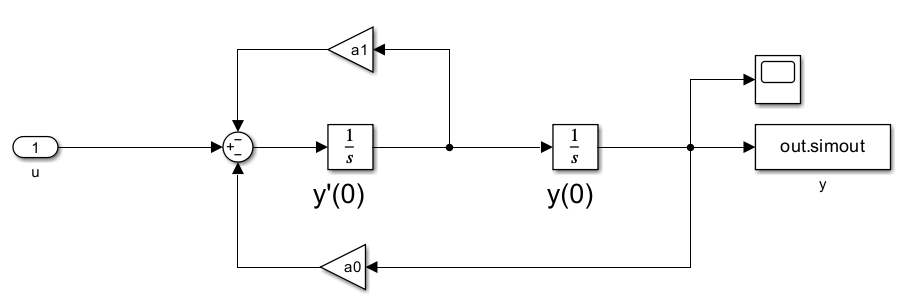
\includegraphics[width=1\textwidth]{scheme_system1.png}
	\caption{Структурная схема - система 2-го порядка}
\end{figure}
\newpage
\section{1-й эксперимент}
Системы описывается следующими коэффициентами:
$$
a_0 = 16.36; a_1 = 1.2
$$
Проведём со следующими входными воздействиями последовательно:
$$
\begin{aligned}
    u_1(t) = 0.5, \\
    u_2(t) = 0.8t, \\
    u_3(t) = sin(2t) 
\end{aligned}
$$
При различных начальных условиях, они будут дублироваться дальше, поэтому напишу их только один раз:
$$
\begin{aligned}
    y(0) = -1, \dot{y}(0)=0; \\
    y(0) = 0, \dot{y}(0)=0; \\
    y(0) = 1, \dot{y}(0)=0; 
\end{aligned}
$$
Получим три выхода:
\begin{figure}[ht]
    \centering
    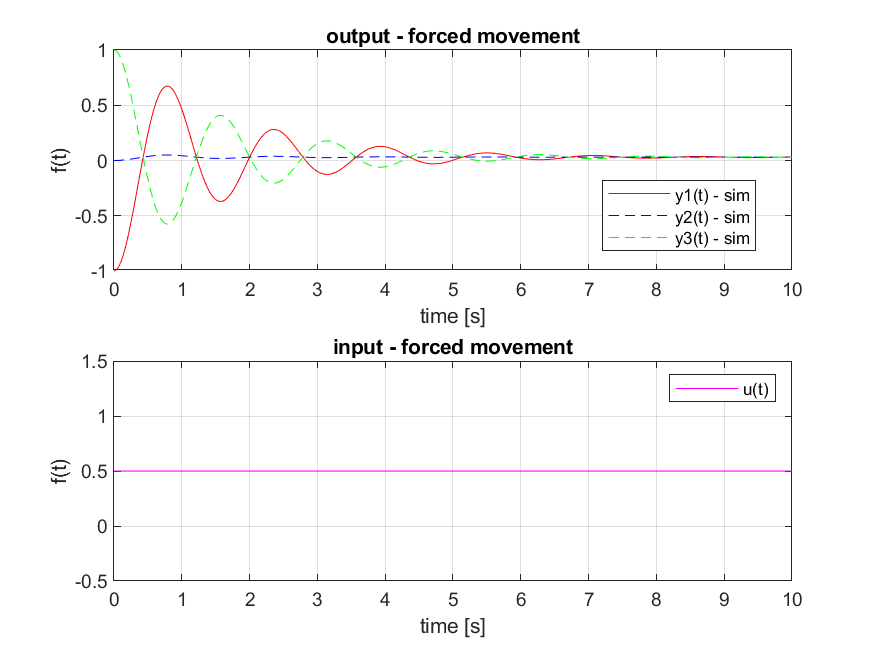
\includegraphics[width=0.8\textwidth]{output_task1_exp11.png}
  \caption{Симуляция - вход $u_1(t)$}
\end{figure}
\begin{figure}[ht]
    \centering
    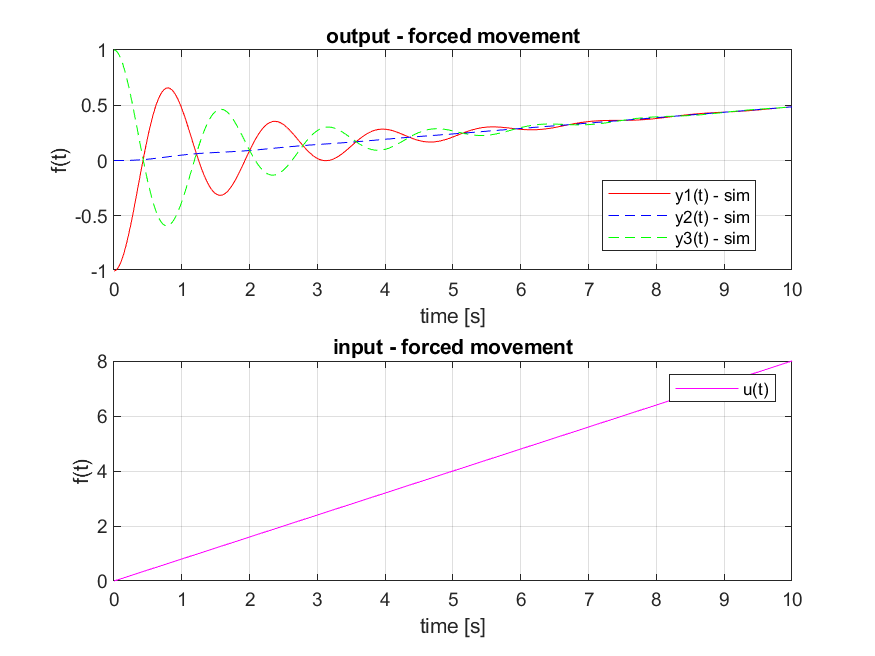
\includegraphics[width=0.8\textwidth]{output_task1_exp12.png}
  \caption{Симуляция - вход $u_2(t)$}
\end{figure}
\begin{figure}[ht]
    \centering
    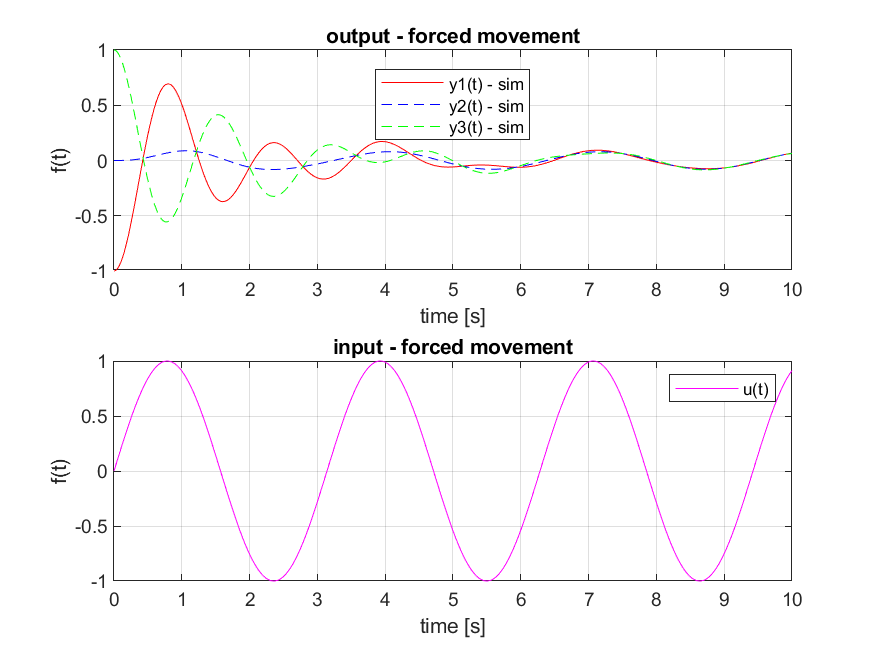
\includegraphics[width=0.8\textwidth]{output_task1_exp13.png}
  \caption{Симуляция - вход $u_3(t)$}
\end{figure}

\newpage
\section{2-й эксперимент}
Системы описывается следующими коэффициентами:
$$
a_0 = 16; a_1 = 0
$$
Проведём со следующими входными воздействиями последовательно:
$$
\begin{aligned}
    u_1(t) = 0.5, \\
    u_2(t) = 0.8t, \\
    u_3(t) = sin(2t) 
\end{aligned}
$$
Получим три выхода:
\begin{figure}[ht]
    \centering
    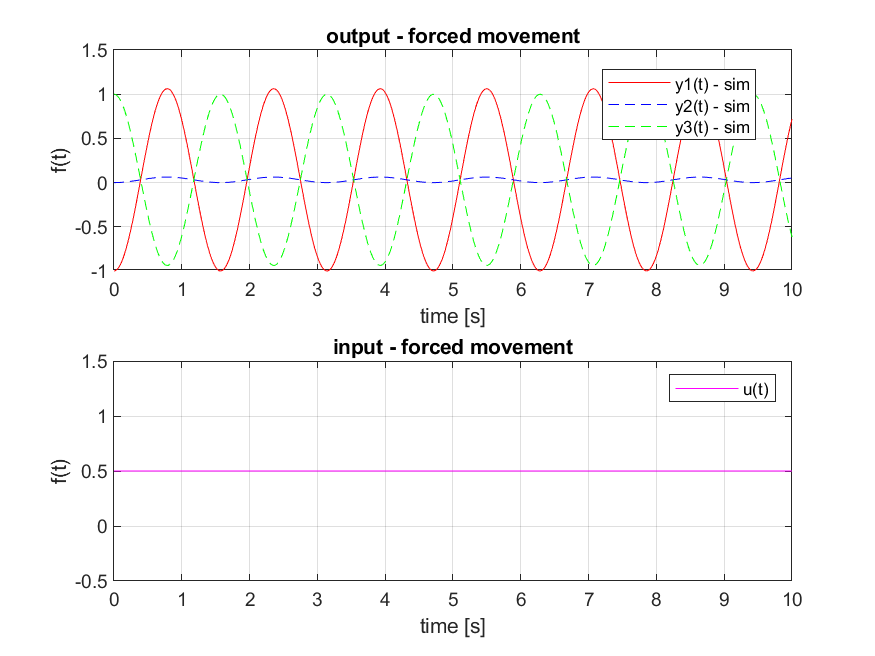
\includegraphics[width=0.8\textwidth]{output_task1_exp21.png}
  \caption{Симуляция - вход $u_1(t)$}
\end{figure}
\begin{figure}[ht]
    \centering
    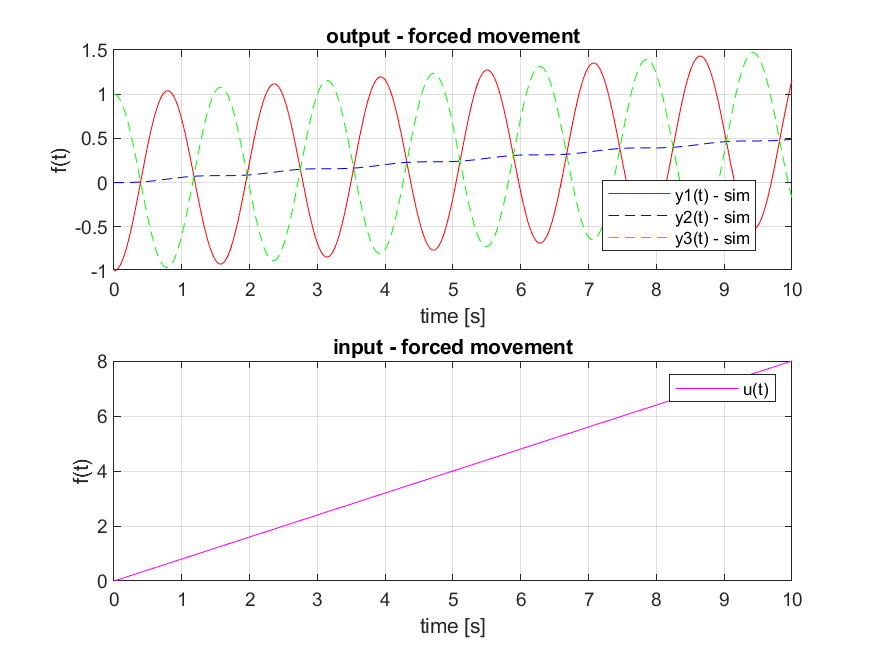
\includegraphics[width=0.8\textwidth]{output_task1_exp22.png}
  \caption{Симуляция - вход $u_2(t)$}
\end{figure}
\begin{figure}[ht]
    \centering
    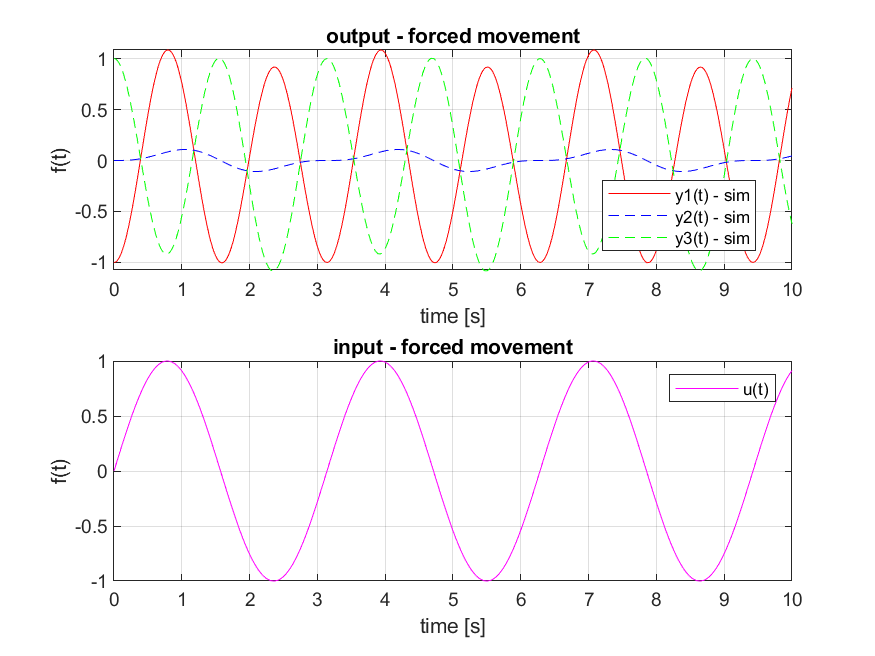
\includegraphics[width=0.8\textwidth]{output_task1_exp23.png}
  \caption{Симуляция - вход $u_3(t)$}
\end{figure}

\newpage
\section{3-й эксперимент}
Системы описывается следующими коэффициентами:
$$
a_0 = 16.36; a_1 = -1.2
$$
Проведём со следующими входными воздействиями последовательно:
$$
\begin{aligned}
    u_1(t) = 0.5, \\
    u_2(t) = 0.8t, \\
    u_3(t) = sin(2t) 
\end{aligned}
$$
Получим три выхода:
\begin{figure}[ht]
    \centering
    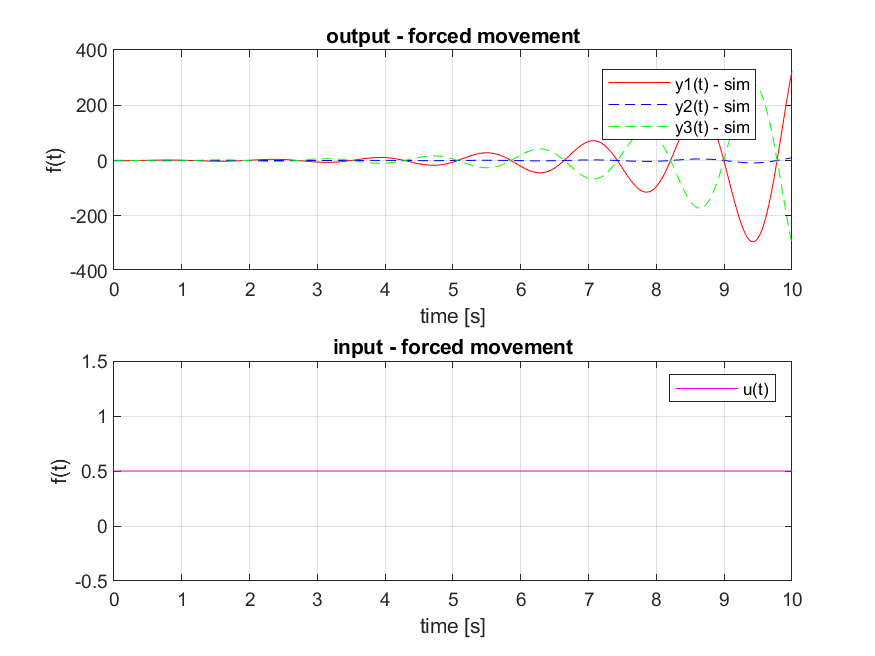
\includegraphics[width=0.8\textwidth]{output_task1_exp31.png}
  \caption{Симуляция - вход $u_1(t)$}
\end{figure}
\begin{figure}[ht]
    \centering
    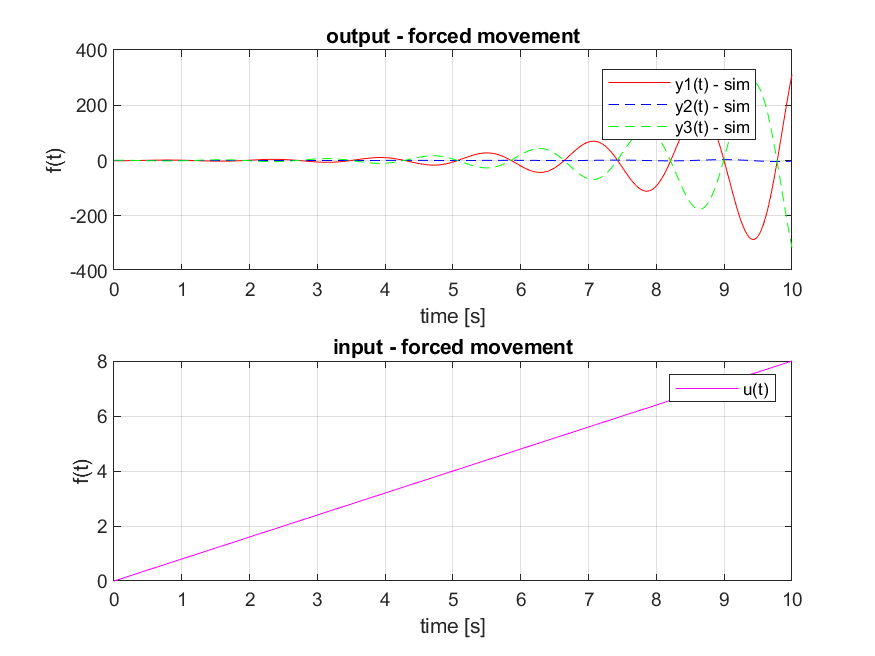
\includegraphics[width=0.8\textwidth]{output_task1_exp32.png}
  \caption{Симуляция - вход $u_2(t)$}
\end{figure}
\begin{figure}[ht]
    \centering
    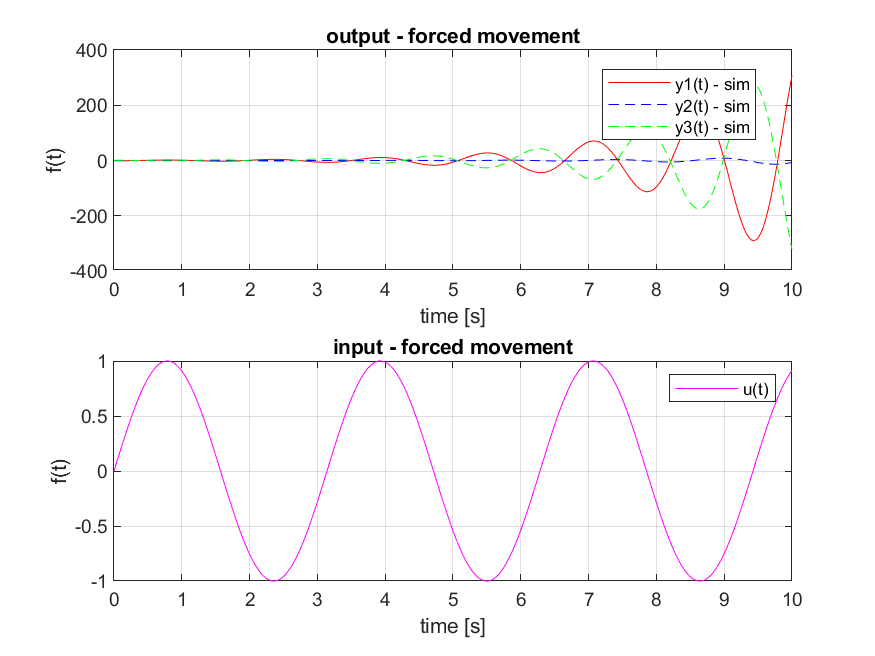
\includegraphics[width=0.8\textwidth]{output_task1_exp33.png}
  \caption{Симуляция - вход $u_3(t)$}
\end{figure}

\section{Выводы}

Каждый выход на рисунке здесь - полное движение, состоящее из свободной и вынужденной части.
Можно заметить тенденцию, что все три графика на одном рисунке сохраняют свою устойчивость, просто из-за различных начальных условий они приходят в устойчивость (или неустойчивость) в разное время, и по-разному. Например, в первом эксперименте все выходы имеют асимптотическую устойчивость, просто "ноль" не всегда совпадает с нулём на графике.
Далее, во втором эксперименте можно заметить устойчивость по Ляпонову, потому что функции будут оставаться всегда в своих рамках. Наконец, в третьем случае, функции будут разбегаться, это уже неустойчивость. П

Из параметров системы ($a_0, a_1$) можно перейти к корневым критериям, которые подтвердят обнаруженные типы устойчивости выше.

Забыл сразу сказать, что начальные условия можно интерпретировать как начальное состояние, то место, откуда мы начинаем двигаться, однако в нашем случае начальные условия не меняют тип устойчивости, хотя в некоторых случаях можно специально подобраться анти-примеры.

\endinput